\documentclass[10pt]{article}

\usepackage[english]{babel}
\usepackage[utf8x]{inputenc}
\usepackage{amsmath}
\usepackage{amssymb}
\usepackage{amsfonts}
\usepackage{graphicx}
\usepackage[ruled]{algorithm2e}
\usepackage{empheq}
\usepackage{float}

\newcommand{\RR}{\mathfrak{R}}
\newcommand{\KK}{\mathfrak{K}}
\newcommand{\CC}{\mathfrak{C}}
\newcommand{\ff}{\mathfrak{f}}

\title{Computing debt cuts leading to global zero-equity - example}

\begin{document}
  \maketitle

\begin{center}
\centerline{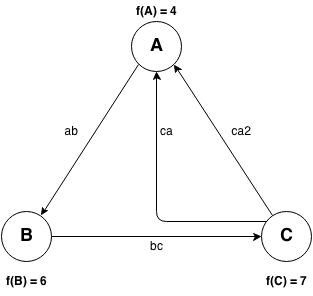
\includegraphics{lce-sample}}
\end{center}
\begin{description}
\item[ab] $(3,0.14,\infty,1)$,
\item[bc] $(2, 0.11, 4, 1.4)$,
\item[ca] $(2.5, 0.05, 6, 0.5)$,
\item[ca2] $(1, 0.27, \infty, 1.7)$.
\end{description}
Equilibrium equation for node $A$:
\begin{align*}
\Xi(ab)e^{0.14 (11.7 - 6)} - \Xi(ca) \Big( 1 + \frac{0.05}{6} \Big)^{ \lfloor 6 (11.7 - 4) \rfloor } - \Xi(ca2) e^{0.27 (11.7 - 4)} &= \\
\underline{2.221 \, \Xi(ab) - 1.464 \, \Xi(ca) - 7.996 \, \Xi(ca2)} &= \\
\CC_{T_G} ( 3e^{ 0.14(6 - 1) }, 0.14, \infty, 6 ) &- \\
\CC_{T_G} ( 2.5 \Big( 1 + \frac{0.05}{6} \Big)^{ \lfloor 6(4 - 0.5) \rfloor }, 0.05, 6, 4 ) &- \\
 \CC_{T_G} ( e^{ 0.27 (4 - 1.7) }, 0.27, \infty, 4 ) &= \\
 \CC_{T_G} (6.041, 0.14, \infty, 6) - \CC_{T_G} ( 2.975, 0.05, 6, 4 ) - \CC_{T_G} ( 1.861, 0.27, \infty, 4 ) &= \\
 13.417 - 4.358 - 14.881 = \underline{-5.822}.
\end{align*}
Equilibrium equation for node $B$:
\begin{align*}
\Xi(bc) \Big( 1 + \frac{0.11}{4} \Big)^{ \lfloor 4(11.7 - 7) \rfloor } - \Xi(ab) e^{0.14( 11.7 - 6 ) } &= \\
\underline{ 1.629 \, \Xi(bc) - 2.221 \, \Xi(ab) } &= \\
\CC_{T_G} (2 \Big( 1 + \frac{0.11}{4} \Big)^{ \lfloor 4(7 - 1.4) \rfloor }, 0.11, 4, 7 ) - \CC_{T_G} ( 3e^{0.14 ( 6 - 1 ) }, 0.14, \infty, 6 ) &= \\
\CC_{T_G} ( 3.632, 0.11, 4, 7 ) - \CC_{T_G} ( 6.041, 0.14, \infty, 6 ) &= \\ 
3.632 \Big( 1 + \frac{0.11}{4} \Big)^{\lfloor 4(11.7 - 7) \rfloor} - 6.041e^{0.14(11.7 - 6)} &= \\
5.918 - 13.417 &= \\
\underline{-7.499}
\end{align*}
Equilibrium equation for node $C$:
\begin{align*}
\Xi(ca) \Big( 1 + \frac{0.05}{6} \Big)^{ \lfloor 6 ( 11.7 - 4) \rfloor } + \Xi(ca2) e^{ 0.27(11.7 - 4) } - \Xi(bc) \Big( 1 + \frac{0.11}{4} \Big)^{ \lfloor 4 (11.7 - 7) \rfloor } &= \\
\underline{1.464 \, \Xi(ca) +7.996 \, \Xi(ca2) - 1.629 \, \Xi(bc)} &= \\
\CC_{T_G} ( 2.5 \Big( 1 + \frac{0.05}{6} \Big)^{ \lfloor 6 ( 4 - 0.5 ) \rfloor }, 0.05, 6, 4) + \CC_{T_G} ( e^{ 0.27 (4 - 1.7) }, 0.27, \infty, 4 ) &- \\
\CC_{T_G} ( 2 \Big( 1 + \frac{0.11}{4} \Big)^{ 4 (7 - 1.4) }, 0.11, 4, 7 ) &= \\
\CC_{T_G} (2.976, 0.05, 6, 4) + \CC_{T_G} ( 1.861, 0.27, \infty, 4 ) - \CC_{T_G} ( 3.633, 0.11, 4, 7 ) &= \\
4.359 + 14.881 - 5.920 &= \\
\underline{13.32}
\end{align*}
Next, the matrix:
\[
\begin{bmatrix}
2.221 & 0 & -1.464 & -7.996 & -5.822 \\
-2.221 & 1.629 & 0 & 0 & -7.499 \\
0 & -1.629 & 1.464 & 7.996 & 13.32 \\
\end{bmatrix}.
\]
Add the first row to the second one:
\[
\begin{bmatrix}
2.221 & 0 & -1.464 & -7.996 & -5.822 \\
0 & 1.629 & -1.464 & -7.996 & -13.32 \\
0 & -1.629 & 1.464 & 7.996 & 13.32 \\
\end{bmatrix}.
\]
Now add the second row to the third:
\[
\begin{bmatrix}
2.221 & 0 & -1.464 & -7.996 & -5.822 \\
0 & 1.629 & -1.464 & -7.996 & -13.32 \\
0 & 0 & 0 & 0 & 0 \\
\end{bmatrix}.
\]
Divide the 1st row by $2.221$:
\[
\begin{bmatrix}
1 & 0 & -0.659 & -3.600 & -2.621 \\
0 & 1.629 & -1.464 & -7.996 & -13.32 \\
0 & 0 & 0 & 0 & 0 \\
\end{bmatrix}.
\]
Divide the 2nd row by $1.629$:
\[
\begin{bmatrix}
1 & 0 & -0.659 & -3.600 & -2.621 \\
0 & 1 & -0.899 & -4.908 & -8.177 \\
0 & 0 & 0 & 0 & 0 \\
\end{bmatrix}.
\]
\end{document}